\section{Application Security Basics}

\subsection{HTTP Basics}

HTTP ist \textbf{Zustandslos}: Der Client sendet eine Anfrage (\textbf{Request}) an den Server, welcher ihn verarbeitet und anschliessend das Resultat als Antwort (\textbf{Response}) zurücksendet.\\

\begin{figure}[H]
	\centering
	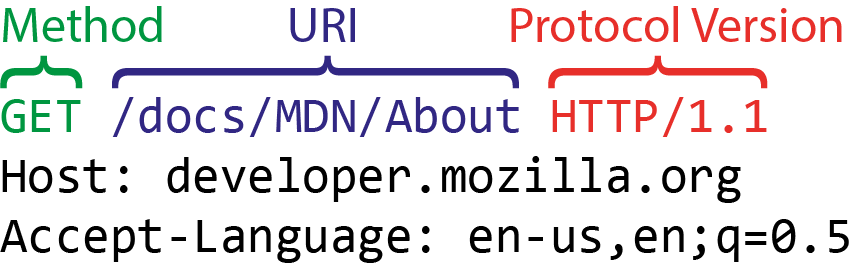
\includegraphics[width=0.38\textwidth]{./img/http-head}
	\caption{HTTP Header}
\end{figure}

Zwischen HTTP GET und POST gibt es einen wesentlichen Unterschied. Da der Server die URI in der Regel mitloggt, werden auch die \textbf{Parameter des GET-Request mitgeloggt}. Beim POST-Request geschieht dies nicht, da sich die Parameter anstatt in der URI im Body befinden. Dies ist auch bei Proxies zu beachten. Eine \textbf{Response} ist beinahe Identisch zum Request. Die erste Zeile enthält nun das Protokoll, Statuscode und Statusbeschreibung (HTTP/1.1 200 OK).

\begin{figure}[H]
	\centering
	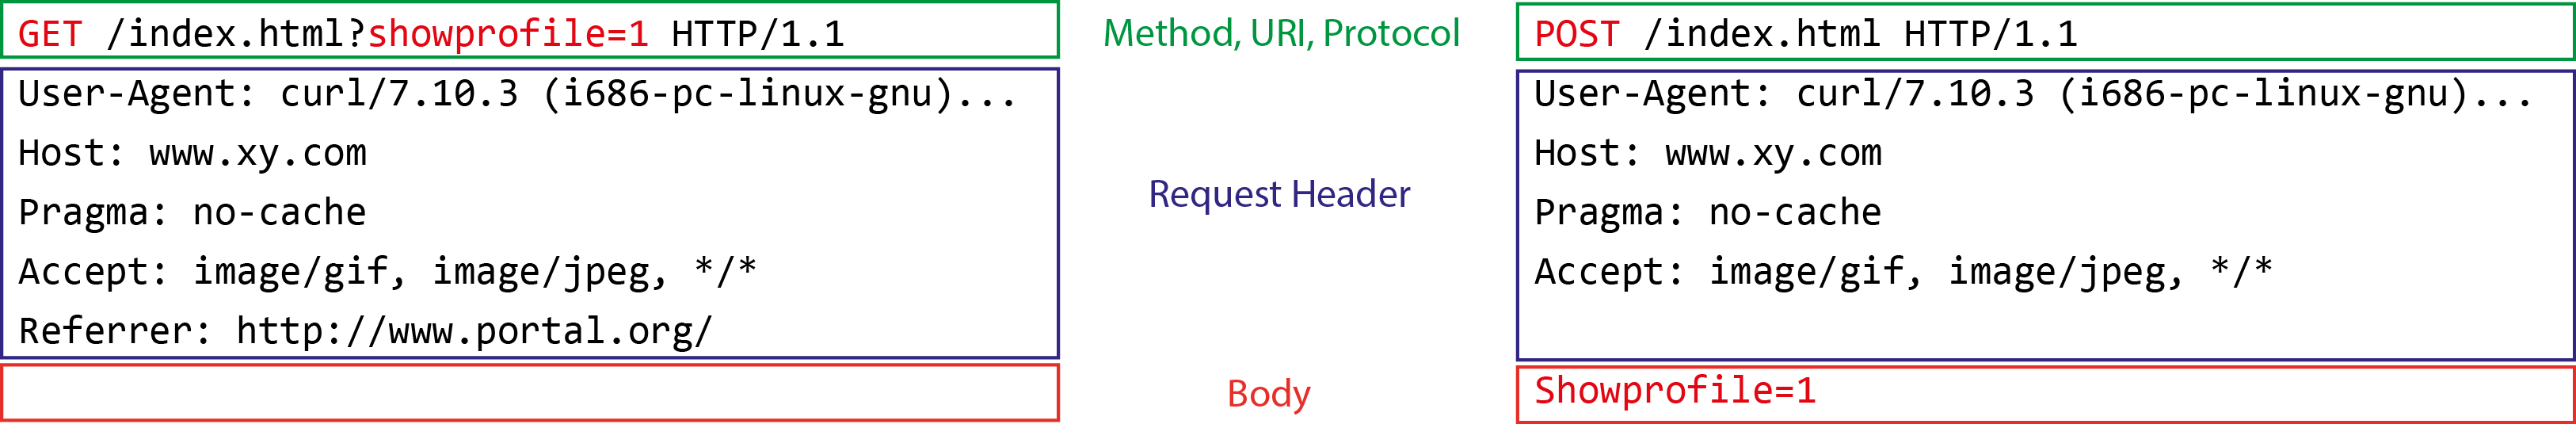
\includegraphics[width=\textwidth]{./img/http-full-request}
	\caption{Beispielrequests für GET und POST}
\end{figure}

\begin{table}[H]
	\begin{tabularx}{\textwidth}{l|X}
		\textbf{HTTP Methode} & \textbf{Verwendung}\\ \hline
		GET		& normale verwendung *\\ \hline
		POST	& übermittlung von Daten (Login, Formulare) *\\ \hline
		HEAD	& Suchmaschinen (Head of page) *\\ \hline
		PUT		& Upload von Dateien (webdav, RESTful)\\ \hline
		DELETE	& Löschen von Dateien (webdav, RESTful)\\ \hline
		OPTIONS	& Auflistung verfügbarer Methoden auf Server\\ \hline
		TRACE	& Debugging in Webserver\\ \hline
	\end{tabularx}
	\caption{Übliche HTTP Methoden (* meist verwendet)}
\end{table}


\begin{table}[H]
	\begin{tabularx}{\textwidth}{l|p{100pt}|X}
		\textbf{Statuscode} & \textbf{Nachricht} & \textbf{Bedeutung}\\ \hline
		\multicolumn{3}{c}{2xx - Erfolgreich} \\ \hline
		200 & OK & Anfrage erfolgreich bearbeitet, Ergebnis in der Antwort enthalten. \\ \hline
		\multicolumn{3}{c}{3xx - Umleitung} \\ \hline
		301 & Moved Permanently & Header "'Location: http://other-site/"' \\ \hline
		302 & Moved Temporarily & Header "'Location: http://other-site/"'; Alternativ 303 oder 307 möglich \\ \hline
		\multicolumn{3}{c}{4xx - Clientfehler} \\ \hline
		400 & Bad Request & Anfrage war fehlerhaft aufgebaut \\ \hline
		401 & Unauthorized & Authentifizierung nötig \\ \hline
		403 & Forbidden & Mangelnde Berechtigung des Clients \\ \hline
		404 & Not Found & Angeforderte Ressource nicht gefunden \\ \hline
		405 & Method Not Allowed & \\ \hline
		408 & Request Timeout & \\ \hline
		\multicolumn{3}{c}{5xx - Serverfehler} \\ \hline
		500 & Internal Server Error & Allgemeiner Serverfehler \\ \hline
		501 & Not Implemented & Funktionalität wird vom Server nicht bereitgestellt \\ \hline
		502 & Bad Gateway & Proxy hat ungültige Antwort erhalten \\ \hline
		503 & Service Unavailable & Service steht temporär nicht zur verfügung \\ \hline
	\end{tabularx}
	\caption{Übliche HTTP Statuscodes,   \href{https://de.wikipedia.org/wiki/HTTP-Statuscode}{Ausführliche Liste auf Wikipedia}}
\end{table}


\todo[inline]{Redirect after successful login}
\todo[inline]{Cookies \& Javascript}
\todo[inline]{Session Handling}
\todo[inline]{Same Origin Policy}
\todo[inline]{CORS}